\documentclass[english,12pt,twoside]{article}

\input{../../131/StudentGuideModule1/labmanual_formatting_commands} %all general latex packages, commands, and definitions now here.

%The \includeonly line below is a great way to save time so you don't always have to compile the WHOLE latex document, if for instance you've only made changes to a single lab.  If you want to compile more than two labs, the syntax is \includeonly{lab1,lab2,lab3} with no spaces after the commas.
%The master.pdf produced will have only the title page, TOC, and that single lab, though the other lab names will appear in the TOC.
%\includeonly{appendices/circuits_to_know/circuits_to_know}

%Use the following line to override all of the 1's and 0's in the \includelab statements below
%\includealllabstrue

\makeindex

\ForceSectionOddPage

\begin{document}

%\newgeometry{total={8in,10.5in},hoffset=0.2in,voffset=0.3in}
\newgeometry{total={8.5in,11in},hoffset=0in,voffset=0in}
%nb: I just messed with the numbers above until it looked okay.  I really don't know what I'm doing. --MT, 4/23/2016
\thispagestyle{empty}
\definecolor{darkblue}{RGB}{0,0,160}
\definecolor{lighterblue}{RGB}{0,128,255} %Looks better on the print shop's printer
\newpagecolor{lighterblue}

%\begin{center}\includegraphics[width=8.5in,trim={0 0 .1cm 0},clip]{electronics_front_pages/electronics_front_cover.eps}
\begin{center}
\includegraphics[width=8.44in]{electronics_front_pages/electronics_front_cover_kuri.eps}
\index{color page}
\end{center}
\newpage

\restoregeometry
\restorepagecolor
\thispagestyle{empty}

\
\vfill
%\textit{Cover art: A randomly chosen, impressive-looking circuit.  You won't build one of these, but you'll do plenty of other cool stuff.}
\textit{Cover art: The circuit diagram from the final class project of a student who took this course in a previous year.  By the end of this course, you will understand all of the components in this diagram and will be able to design and build similar circuits  yourself.}
\pagebreak



\title{Electronics For Doing!\\
Laboratory Exercises for Physics 216}

\author{Matthew L. Trawick\\[4pt]
Department of Physics, University of Richmond, VA \\[4pt]
}

\maketitle

\vspace{0.4 in}

%\begin{abstract}

\begin{center}
\large{\textbf{Welcome to Electronics!}}
\end{center}

The exercises in this manual are for a course in electronics that emphasizes active learning. 
Sitting passively and listening to lectures is boring, and doesn't help you learn very well either.
Instead, this manual will guide you through a series of exercises designed to help you learn things by yourself as you go along, interrupted by me only occasionally to explain some of the tricky parts.

As you work, think about what you're supposed to be learning with each exercise.  If an exercise shows you a circuit that does X, then you should walk away from the lab knowing exactly how to build a circuit that does X.  Presumably, you'll be asked to do so on an exam soon enough!

Your written work will be done in a separate lab notebook.  For each numbered part, you should document your work with a quick circuit diagram or note about what you did, and include any data you take and any conclusions you draw.  Also, any sentence in this manual that ends with a question mark needs to be answered by you in your notebook.

Electronics is fun!  Don't be afraid to experiment!  The worst that can happen is you light some components on fire.  (No worries---they're not yours!)

Enjoy the ride and be excellent,

---Matt Trawick
%\end{abstract}


\newpage
\
\thispagestyle{plain}

\newpage
\




\tableofcontents{}
\cleardoublepage
\renewcommand{\headersupplementmark}{Lab }

%--------------------------------------------
\part{The Basics}

\includelab{1}{equipment/equipment}
\includelab{1}{power/power}
\includelab{1}{voltage_dividers/voltage_dividers}
\includelab{1}{input_output_impedance/input_output_impedance}
\includelab{1}{oscilloscope/oscilloscope}
\includelab{1}{bridge_circuit/bridge_circuit}

%--------------------------------------------
\part{Two Very Important Kinds of Integrated Circuits}

\includelab{1}{op-amps/op-amps}
\includelab{1}{digital_electronics/digital_electronics} %ADD pinouts sometime later

%--------------------------------------------
\part{Capacitors, Inductors, and AC circuits}

\includelab{1}{capacitors/capacitors}
\includelab{1}{transformers/transformers}
\includelab{1}{diodes/diodes}
\includelab{1}{power_supply/power_supply}
\includelab{1}{inductors/inductors}
\includelab{1}{ac_circuits/ac_circuits}
\includelab{1}{filters/filters}

%--------------------------------------------
\part{Relays and Transistors}

\includelab{1}{relays/relays}
\includelab{1}{bjt/bjt}
\includelab{1}{multisim/multisim}
\includelab{1}{bjt_saturation/bjt_saturation}
\includelab{1}{jfet/jfet}

%--------------------------------------------
\part{Sensors, Some Special Purpose Chips, and Applications}

\includelab{1}{microphone_photocell/microphone_photocell}
\includelab{1}{flipflops/flipflops}
\includelab{1}{timers/timers}
\includelab{1}{counters/counters}
\setcounter{section}{98} %set this to desired next section number MINUS ONE
\includelab{1}{lab_99/lab_99}

%--------------------------------------------
%\part{Appendices}
\immediateaddcontentsline{toc}{part}{Appendices} %Avoids a Roman part number for the Appendices in the toc
\appendix
\renewcommand{\headersupplementmark}{Appendix }
\titleformat{\section}{\normalfont\large\bfseries}{\headersupplementmark \thesection :}{1ex}{}

%\cleardoublepage
%\NoForceSectionOddPage

\includelab{1}{appendices/pinouts/pinouts}
\includelab{1}{appendices/one_page_uncertainty/one_page_uncertainty_electronics}
%\includelab{1}[../../131/StudentGuideModule1/]{appendices/one_page_uncertainty/one_page_uncertainty}
\includelab{1}{appendices/oscilloscope_checklist/oscilloscope_checklist}
\includelab{1}{appendices/circuits_to_know/circuits_to_know}
%\includelab{1}[../../132/StudentGuideModule2/]{electric_circuits/electric_circuits}
%\includelab{1}[../../132/StudentGuideModule2/]{electric_circuits2/electric_circuits2}

\end{document}
